\section{Results}
\begin{frame}{The pp-chain}
    \begin{figure}
        \centering
        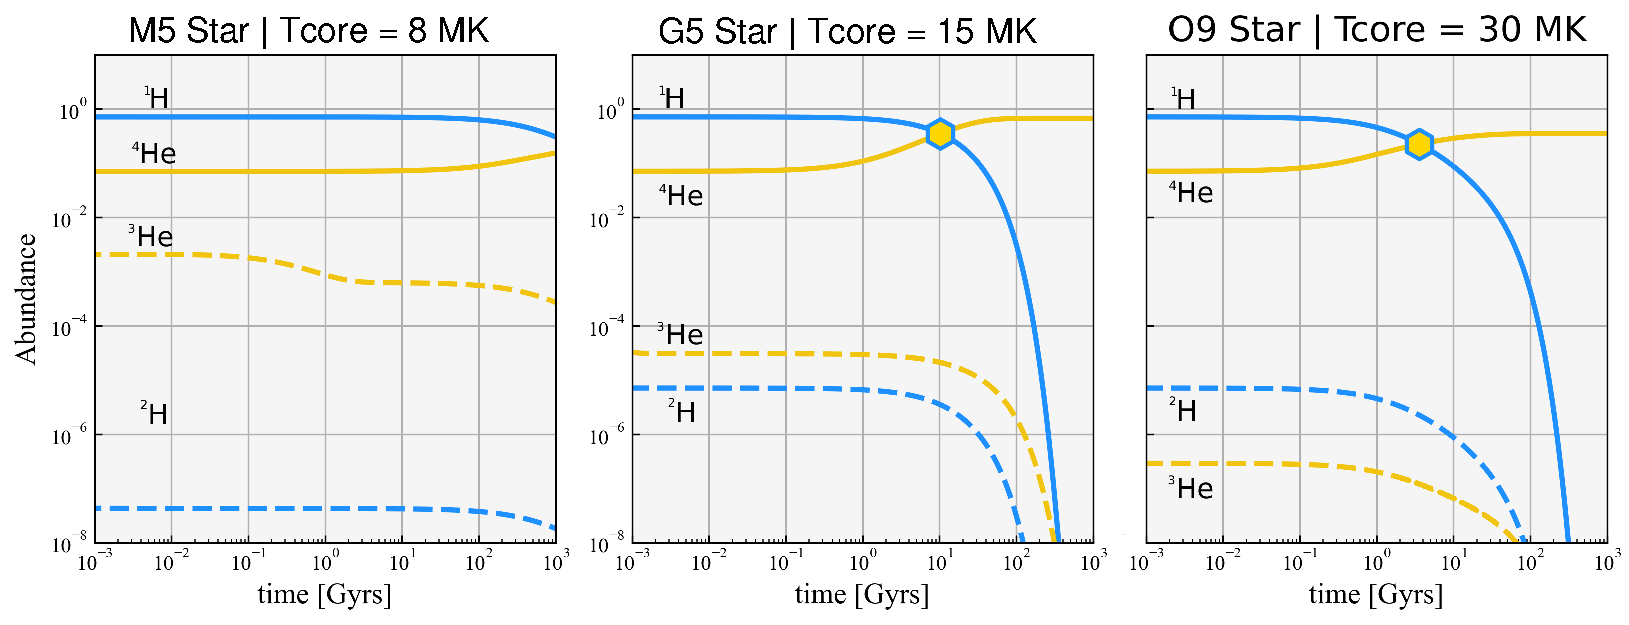
\includegraphics[width = 1\textwidth]{figs/ppCHAIN_FINAL.pdf}
        \caption{Nuclear fusion via the pp-chain for a M5, G5, and O9 star.}
        \label{fig:enter-label}
    \end{figure}
    \begin{itemize}
        \item<2->Higher $T\rightarrow$ more fusion $\Rightarrow$ Hotter stars live shorter
        \item<3->Abundances reach an equilibrium
        \item<4->${}^\text{1}$H-${}^\text{4}$He equality roughly correspond to star lifetime
    \end{itemize}
\end{frame}

\begin{frame}{The CNO-cycle}
\begin{columns}
    \begin{column}{0.8\textwidth}
    \begin{figure}
        \centering
        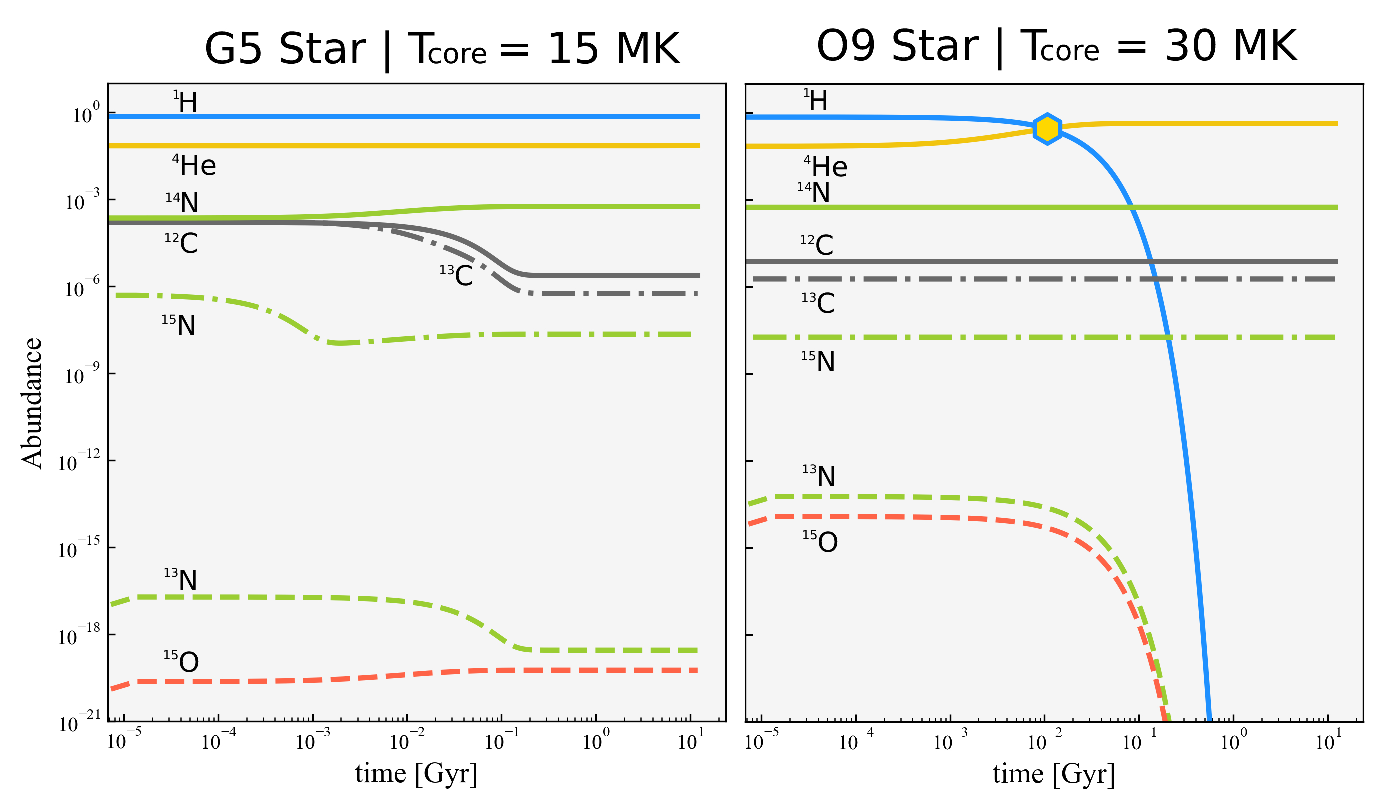
\includegraphics[width = 1\textwidth]{figs/cno2.pdf}
        \caption{Nuclear fusion via the CNO-cycle for a G5 and O9 star.}
        \label{fig:enter-label}
    \end{figure}

    \end{column}
    \begin{column}{0.2\textwidth}
        \only<3->{
        \begin{align*}
             {}^\text{12}\text{C} + {}^\text{1}\text{H} &\rightarrow {}^\text{13}\text{N}  \\
             {}^\text{13}\text{N} &\rightarrow {}^\text{13}\text{C} \\
             {}^\text{13}\text{C} + {}^\text{1}\text{H} &\rightarrow {}^\text{14}\text{N} \\
             {}^\text{14}\text{N} + {}^\text{1}\text{H} &\rightarrow {}^\text{15}\text{O} \\
             {}^\text{15}\text{O} &\rightarrow {}^\text{15}\text{N} \\
             {}^\text{15}\text{N} + {}^\text{1}\text{H} &\rightarrow {}^\text{12}\text{C} + {}^\text{4}\text{He}
        \end{align*}
        }
    \end{column}
\end{columns}
    \only<2>{Similarities to pp-chain \begin{itemize}
        \item Higher $T\rightarrow$ more fusion $\Rightarrow$ Hotter stars live shorter
        \item Abundances reach an equilibrium
    \end{itemize}}
    \begin{itemize}
        \item<4->Once ${}^\text{1}$H runs out, only decay reactions occur
        \item<5->Catalysts become constant in the long run
    \end{itemize}
\end{frame}

\begin{frame}{pp-chain vs CNO-cycle}
    \only<1>{\centering \large pp-chain vs CNO-cycle\\ \LARGE Which one dominates when?}
    \only<2>{
        What we expect:
            \begin{figure}
                \centering
                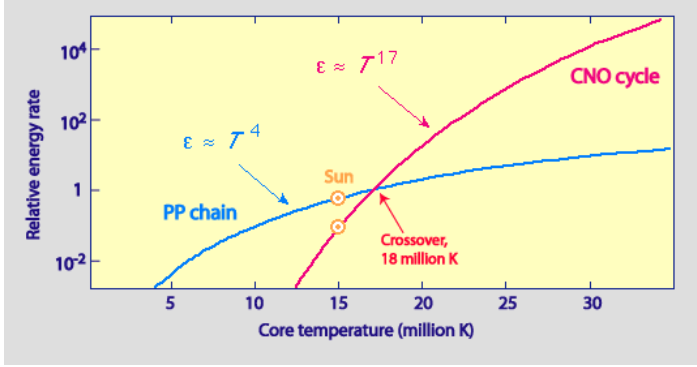
\includegraphics[width = 0.9\textwidth]{figs/cross.png}
                \caption{Source: Mike Guidry, University of Tennessee}
                \label{fig:enter-label}
            \end{figure}
        }
    \only<3>{
    What we got:
        \begin{figure}
            \centering
            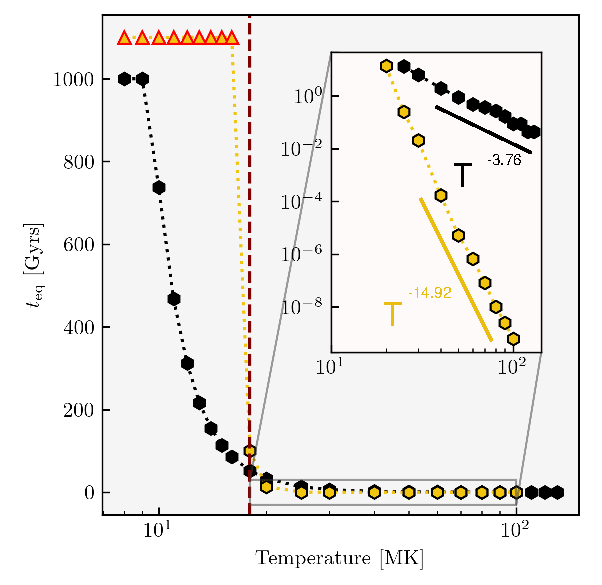
\includegraphics[height=0.75\textheight]{figs/FINAL_FOR_REAL_teq_T.pdf}
            \caption{${}^\text{1}$H-${}^\text{4}$He equality time for pp-chain and CNO-cycle across temperatures}
            \label{fig:enter-label}
        \end{figure}
        }

\end{frame}

\begin{frame}{Temperature and metallicity}
    % \centering
    % $\left[\begin{tabular}{c}
    % Super awesome slide with the phase-diagram, \\ which totally was not a pain in the ass to make \\ and made my life expectancy drop by 10\%
    % \end{tabular}\right]$
    \only<1>{\centering \large That was for ISM abundances\\ \LARGE How does metallicity change the game?}
    \only<2->{
    \begin{figure}
        \centering
        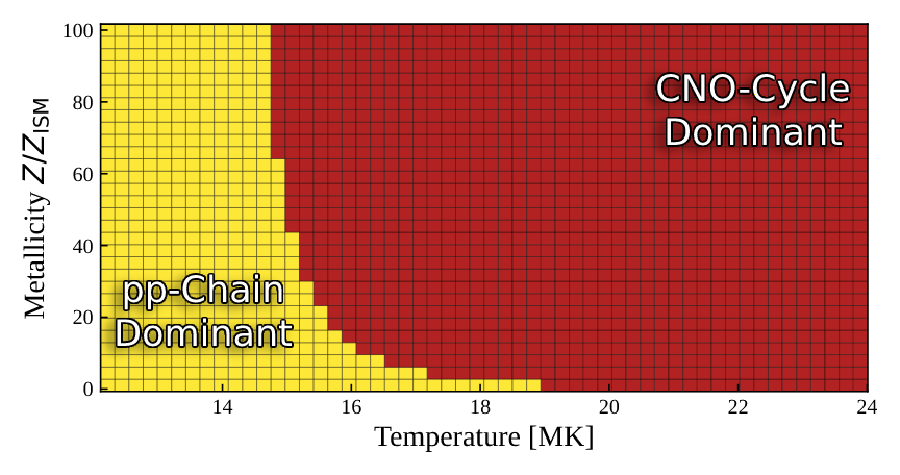
\includegraphics[height=0.75\textheight]{figs/Dominance.pdf}
        \caption{Which fusion pathway dominates at which $(T_\mathrm{core}, Z)$}
        \label{fig:enter-label}
    \end{figure}
    }
\end{frame}